\section{TÌM KIẾM NGỮ NGHĨA}
\subsection{Tổng quan}
\hspace*{1cm}Tìm kiếm ngữ nghĩa là một công cụ search thông qua việc phân tích các từ ngữ và các cụm từ, trả về kết quả có nội dung các từ tương đồng với ngữ nghĩa các từ khóa xuất hiện trong câu truy vấn thay vì phải trùng khớp từng từ, sử dụng trí tuệ nhân tạo để hiểu ý nghĩa của truy vấn và mối quan hệ giữa các từ để trả về những kết quả phù hợp và chính xác hơn.\\
\hspace*{1cm}Tìm kiếm ngữ nghĩa được vận hành dựa trên vector search cho phép semantic search để có thể tìm kiếm và sắp xếp thông tin dựa trên các nội dung liên quan. Vector search mã hóa các chi tiết của thông tin tìm kiếm thành các trường có liên quan hoặc các vector để có thể so sánh các vector và tìm kiếm sự tương đồng giữa chúng
\begin{enumerate}
    \item Khi một câu truy vấn được thực hiện, search engine chuyển câu query thành dạng embedding, đại diện bởi dạng dữ liệu số và các nội dung liên quan, lưu trữ vào các vector.
    \begin{figure}[H]
        \centering
        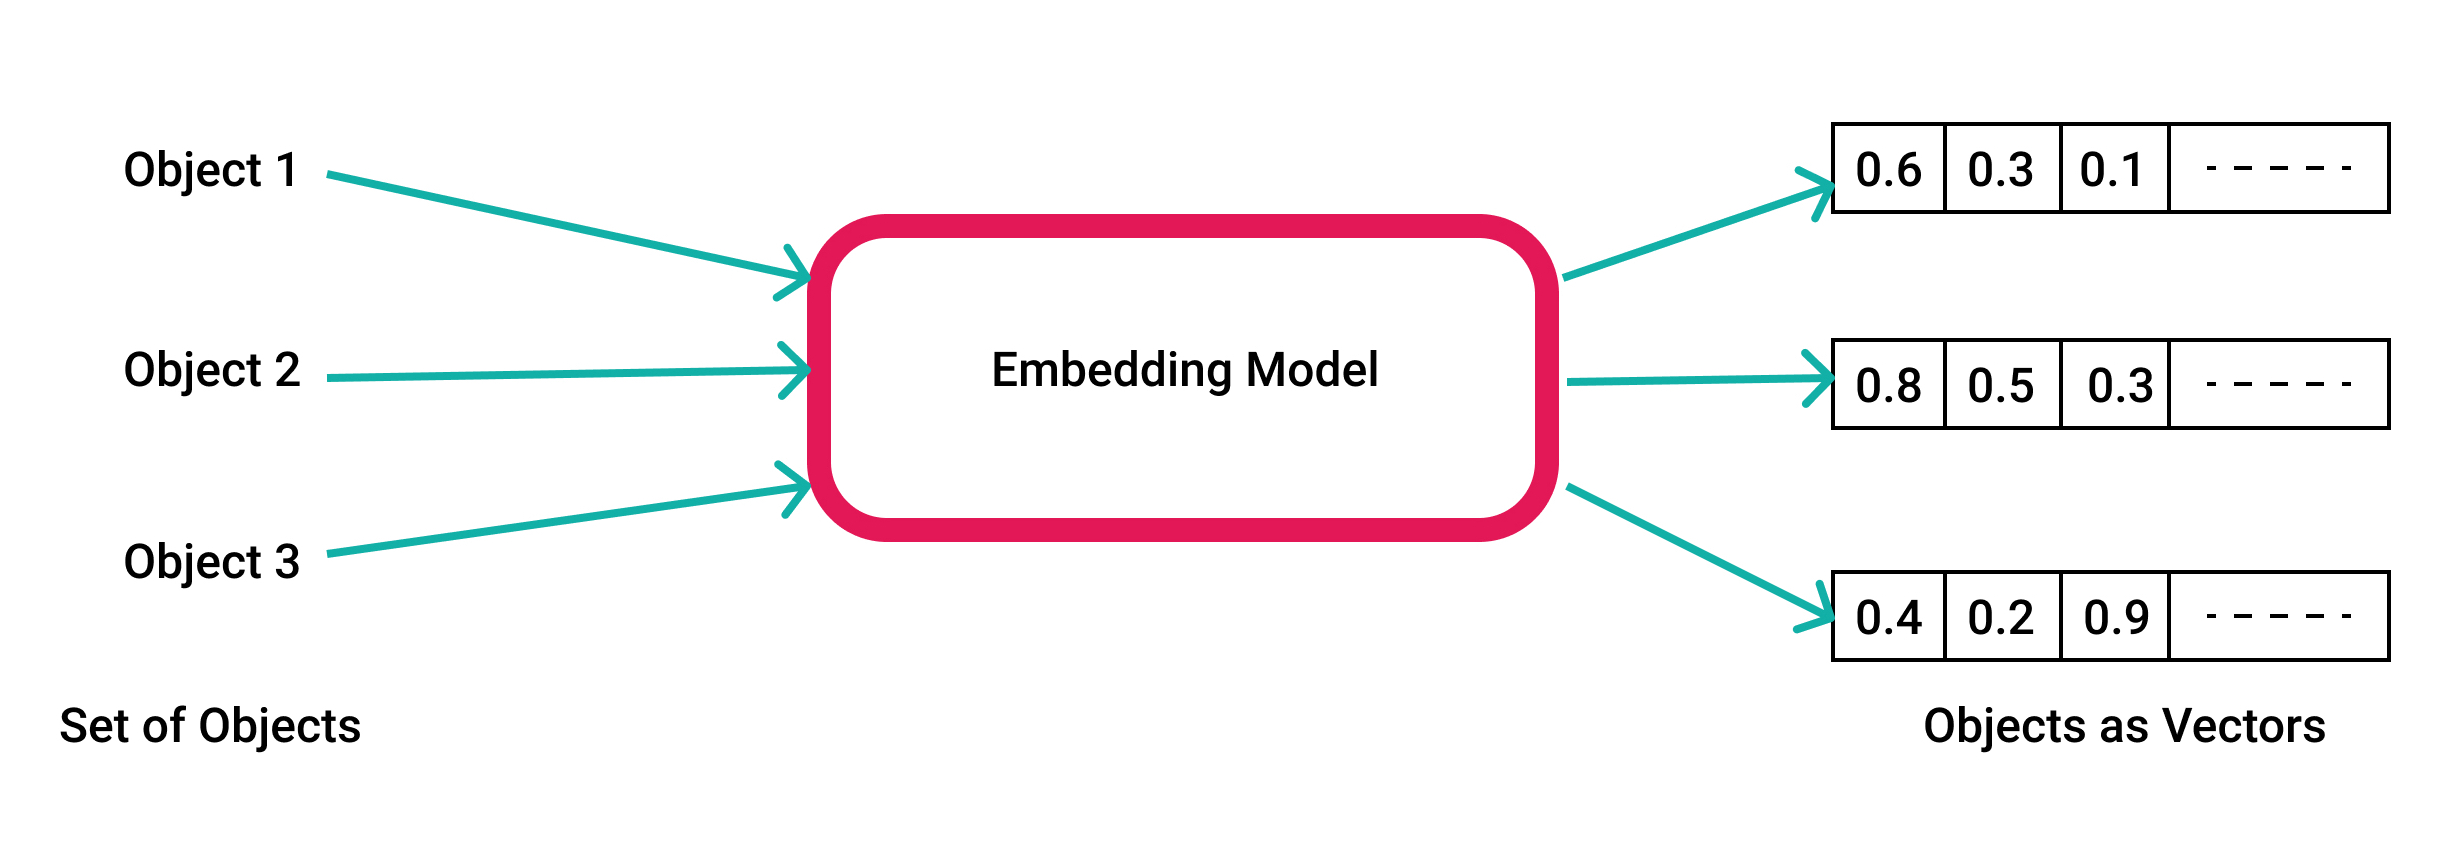
\includegraphics[width=1\textwidth]{Images/embedding.png}
        \caption{Vector embedding}
        \label{fig:ftsexample}
    \end{figure}
    \item Sử dụng Cosine Similarity để tìm các vector chứa các nội dung liên quan đến vector câu truy vấn.
\end{enumerate}
\textbf{Ví dụ:} khi bạn sử dụng tìm kiếm ngữ nghĩa để tìm kiếm "\textbf{nhà hàng gần đây}", nó sẽ không chỉ trả về danh sách các nhà hàng có chứa từ khóa "\textbf{nhà hàng}" và "\textbf{gần đây}", mà còn xem xét các yếu tố khác như vị trí hiện tại, loại nhà hàng bạn thích, và đánh giá của khách hàng.
\subsection{Phân tích ưu và nhược điểm}
\textbf{Ưu điểm}
\begin{itemize}
    \item \textbf{Kết quả chính xác hơn:} giúp người dùng tìm thấy thông tin phù hợp với nhu cầu hơn, vì nó xem xét ý nghĩa và ngữ cảnh của truy vấn.
    \item \textbf{Có thể tìm kiếm thông tin phức tạp:} có thể hiểu được các truy vấn phức tạp và trả về những kết quả phù hợp.
    \item \textbf{Ít phụ thuộc vào từ khóa:} Không cần phải sử dụng những từ khóa chính xác để tìm kiếm thông tin. Thay vào đó, có thể sử dụng ngôn ngữ tự nhiên để diễn đạt truy vấn của mình.
\end{itemize}
\textbf{Nhược điểm}
\begin{itemize}
    \item \textbf{Yêu cầu công nghệ cao:} đòi hỏi phải có công nghệ trí tuệ nhân tạo, học máy để việc tìm kiếm hiệu quả hơn, do đó có thể khá tốn kém và khó khăn để triển khai.
    \item \textbf{Kết quả có thể không chính xác hoàn toàn:} Mặc dù đã được cải tiến rất nhiều, nhưng nó vẫn có thể trả về những kết quả không chính xác hoàn toàn điều này phụ thuộc rất nhiều vào độ chính xác của các mô hình được sử dụng
    \item \textbf{Thiếu dữ liệu:} hoạt động hiệu quả nhất khi có nhiều dữ liệu để phân tích. Nếu không có đủ dữ liệu, có thể không hiểu được ý nghĩa của truy vấn và trả về những kết quả không chính xác.
\end{itemize}